\documentclass[twoside]{book}

% Packages required by doxygen
\usepackage{fixltx2e}
\usepackage{calc}
\usepackage{doxygen}
\usepackage[export]{adjustbox} % also loads graphicx
\usepackage{graphicx}
\usepackage[utf8]{inputenc}
\usepackage{makeidx}
\usepackage{multicol}
\usepackage{multirow}
\PassOptionsToPackage{warn}{textcomp}
\usepackage{textcomp}
\usepackage[nointegrals]{wasysym}
\usepackage[table]{xcolor}

% Font selection
\usepackage[T1]{fontenc}
\usepackage[scaled=.90]{helvet}
\usepackage{courier}
\usepackage{amssymb}
\usepackage{sectsty}
\renewcommand{\familydefault}{\sfdefault}
\allsectionsfont{%
  \fontseries{bc}\selectfont%
  \color{darkgray}%
}
\renewcommand{\DoxyLabelFont}{%
  \fontseries{bc}\selectfont%
  \color{darkgray}%
}
\newcommand{\+}{\discretionary{\mbox{\scriptsize$\hookleftarrow$}}{}{}}

% Page & text layout
\usepackage{geometry}
\geometry{%
  a4paper,%
  top=2.5cm,%
  bottom=2.5cm,%
  left=2.5cm,%
  right=2.5cm%
}
\tolerance=750
\hfuzz=15pt
\hbadness=750
\setlength{\emergencystretch}{15pt}
\setlength{\parindent}{0cm}
\setlength{\parskip}{3ex plus 2ex minus 2ex}
\makeatletter
\renewcommand{\paragraph}{%
  \@startsection{paragraph}{4}{0ex}{-1.0ex}{1.0ex}{%
    \normalfont\normalsize\bfseries\SS@parafont%
  }%
}
\renewcommand{\subparagraph}{%
  \@startsection{subparagraph}{5}{0ex}{-1.0ex}{1.0ex}{%
    \normalfont\normalsize\bfseries\SS@subparafont%
  }%
}
\makeatother

% Headers & footers
\usepackage{fancyhdr}
\pagestyle{fancyplain}
\fancyhead[LE]{\fancyplain{}{\bfseries\thepage}}
\fancyhead[CE]{\fancyplain{}{}}
\fancyhead[RE]{\fancyplain{}{\bfseries\leftmark}}
\fancyhead[LO]{\fancyplain{}{\bfseries\rightmark}}
\fancyhead[CO]{\fancyplain{}{}}
\fancyhead[RO]{\fancyplain{}{\bfseries\thepage}}
\fancyfoot[LE]{\fancyplain{}{}}
\fancyfoot[CE]{\fancyplain{}{}}
\fancyfoot[RE]{\fancyplain{}{\bfseries\scriptsize Generated by Doxygen }}
\fancyfoot[LO]{\fancyplain{}{\bfseries\scriptsize Generated by Doxygen }}
\fancyfoot[CO]{\fancyplain{}{}}
\fancyfoot[RO]{\fancyplain{}{}}
\renewcommand{\footrulewidth}{0.4pt}
\renewcommand{\chaptermark}[1]{%
  \markboth{#1}{}%
}
\renewcommand{\sectionmark}[1]{%
  \markright{\thesection\ #1}%
}

% Indices & bibliography
\usepackage{natbib}
\usepackage[titles]{tocloft}
\setcounter{tocdepth}{3}
\setcounter{secnumdepth}{5}
\makeindex

% Hyperlinks (required, but should be loaded last)
\usepackage{ifpdf}
\ifpdf
  \usepackage[pdftex,pagebackref=true]{hyperref}
\else
  \usepackage[ps2pdf,pagebackref=true]{hyperref}
\fi
\hypersetup{%
  colorlinks=true,%
  linkcolor=blue,%
  citecolor=blue,%
  unicode%
}

% Custom commands
\newcommand{\clearemptydoublepage}{%
  \newpage{\pagestyle{empty}\cleardoublepage}%
}

\usepackage{caption}
\captionsetup{labelsep=space,justification=centering,font={bf},singlelinecheck=off,skip=4pt,position=top}

%===== C O N T E N T S =====

\begin{document}

% Titlepage & ToC
\hypersetup{pageanchor=false,
             bookmarksnumbered=true,
             pdfencoding=unicode
            }
\pagenumbering{roman}
\begin{titlepage}
\vspace*{7cm}
\begin{center}%
{\Large C\+O\+P290-\/\+Assignment1 }\\
\vspace*{1cm}
{\large Generated by Doxygen 1.8.11}\\
\end{center}
\end{titlepage}
\clearemptydoublepage
\tableofcontents
\clearemptydoublepage
\pagenumbering{arabic}
\hypersetup{pageanchor=true}

%--- Begin generated contents ---
\chapter{Namespace Index}
\section{Namespace List}
Here is a list of all namespaces with brief descriptions\+:\begin{DoxyCompactList}
\item\contentsline{section}{\hyperlink{namespaceextra__functions__3dedge}{extra\+\_\+functions\+\_\+3dedge} }{\pageref{namespaceextra__functions__3dedge}}{}
\item\contentsline{section}{\hyperlink{namespaceextra__functions__3dvertex}{extra\+\_\+functions\+\_\+3dvertex} }{\pageref{namespaceextra__functions__3dvertex}}{}
\end{DoxyCompactList}

\chapter{File Index}
\section{File List}
Here is a list of all files with brief descriptions\+:\begin{DoxyCompactList}
\item\contentsline{section}{src/\hyperlink{_edge2d___list_8cpp}{Edge2d\+\_\+\+List.\+cpp} }{\pageref{_edge2d___list_8cpp}}{}
\item\contentsline{section}{src/\hyperlink{_edge3d___list_8cpp}{Edge3d\+\_\+\+List.\+cpp} }{\pageref{_edge3d___list_8cpp}}{}
\item\contentsline{section}{src/\hyperlink{_face3d___list_8cpp}{Face3d\+\_\+\+List.\+cpp} }{\pageref{_face3d___list_8cpp}}{}
\item\contentsline{section}{src/\hyperlink{_hidden_lines_8cpp}{Hidden\+Lines.\+cpp} }{\pageref{_hidden_lines_8cpp}}{}
\item\contentsline{section}{src/\hyperlink{main_8cpp}{main.\+cpp} }{\pageref{main_8cpp}}{}
\item\contentsline{section}{src/\hyperlink{_projection2d_8cpp}{Projection2d.\+cpp} }{\pageref{_projection2d_8cpp}}{}
\item\contentsline{section}{src/\hyperlink{_solid3d_8cpp}{Solid3d.\+cpp} }{\pageref{_solid3d_8cpp}}{}
\item\contentsline{section}{src/\hyperlink{_surface3d___list_8cpp}{Surface3d\+\_\+\+List.\+cpp} }{\pageref{_surface3d___list_8cpp}}{}
\item\contentsline{section}{src/\hyperlink{_vertex2d___list_8cpp}{Vertex2d\+\_\+\+List.\+cpp} }{\pageref{_vertex2d___list_8cpp}}{}
\item\contentsline{section}{src/\hyperlink{_vertex3d___list_8cpp}{Vertex3d\+\_\+\+List.\+cpp} }{\pageref{_vertex3d___list_8cpp}}{}
\end{DoxyCompactList}

\chapter{Namespace Documentation}
\hypertarget{namespaceextra__functions__3dedge}{}\section{extra\+\_\+functions\+\_\+3dedge Namespace Reference}
\label{namespaceextra__functions__3dedge}\index{extra\+\_\+functions\+\_\+3dedge@{extra\+\_\+functions\+\_\+3dedge}}
\subsection*{Functions}
\begin{DoxyCompactItemize}
\item 
bool \hyperlink{namespaceextra__functions__3dedge_ae7c8fa0d6b3476fe882e957553ccdd86}{equal\+\_\+3dedge} (Edge3d e1, Edge3d e2)
\item 
int \hyperlink{namespaceextra__functions__3dedge_a5ad68cbd008f410b737b334315042d56}{edge\+\_\+index} (vector$<$ Edge3d $>$ elist, Edge3d e)
\end{DoxyCompactItemize}


\subsection{Function Documentation}
\index{extra\+\_\+functions\+\_\+3dedge@{extra\+\_\+functions\+\_\+3dedge}!edge\+\_\+index@{edge\+\_\+index}}
\index{edge\+\_\+index@{edge\+\_\+index}!extra\+\_\+functions\+\_\+3dedge@{extra\+\_\+functions\+\_\+3dedge}}
\subsubsection[{\texorpdfstring{edge\+\_\+index(vector$<$ Edge3d $>$ elist, Edge3d e)}{edge_index(vector< Edge3d > elist, Edge3d e)}}]{\setlength{\rightskip}{0pt plus 5cm}int extra\+\_\+functions\+\_\+3dedge\+::edge\+\_\+index (
\begin{DoxyParamCaption}
\item[{vector$<$ Edge3d $>$}]{elist, }
\item[{Edge3d}]{e}
\end{DoxyParamCaption}
)}\hypertarget{namespaceextra__functions__3dedge_a5ad68cbd008f410b737b334315042d56}{}\label{namespaceextra__functions__3dedge_a5ad68cbd008f410b737b334315042d56}


Definition at line 16 of file Edge3d\+\_\+\+List.\+cpp.

\index{extra\+\_\+functions\+\_\+3dedge@{extra\+\_\+functions\+\_\+3dedge}!equal\+\_\+3dedge@{equal\+\_\+3dedge}}
\index{equal\+\_\+3dedge@{equal\+\_\+3dedge}!extra\+\_\+functions\+\_\+3dedge@{extra\+\_\+functions\+\_\+3dedge}}
\subsubsection[{\texorpdfstring{equal\+\_\+3dedge(\+Edge3d e1, Edge3d e2)}{equal_3dedge(Edge3d e1, Edge3d e2)}}]{\setlength{\rightskip}{0pt plus 5cm}bool extra\+\_\+functions\+\_\+3dedge\+::equal\+\_\+3dedge (
\begin{DoxyParamCaption}
\item[{Edge3d}]{e1, }
\item[{Edge3d}]{e2}
\end{DoxyParamCaption}
)}\hypertarget{namespaceextra__functions__3dedge_ae7c8fa0d6b3476fe882e957553ccdd86}{}\label{namespaceextra__functions__3dedge_ae7c8fa0d6b3476fe882e957553ccdd86}


Definition at line 8 of file Edge3d\+\_\+\+List.\+cpp.


\hypertarget{namespaceextra__functions__3dvertex}{}\section{extra\+\_\+functions\+\_\+3dvertex Namespace Reference}
\label{namespaceextra__functions__3dvertex}\index{extra\+\_\+functions\+\_\+3dvertex@{extra\+\_\+functions\+\_\+3dvertex}}
\subsection*{Functions}
\begin{DoxyCompactItemize}
\item 
bool \hyperlink{namespaceextra__functions__3dvertex_a0da949fe0a7c4031ef70dc6f95145845}{vertex3d\+\_\+possible} (Vertex2d front, Vertex2d top, Vertex2d side)
\item 
bool \hyperlink{namespaceextra__functions__3dvertex_a9428b2b2156e274aff497ebd80f5e3a1}{equal\+\_\+3dvertex} (Vertex3d v1, Vertex3d v2)
\item 
Vertex3d \hyperlink{namespaceextra__functions__3dvertex_a8016663b5ddeb59267c20901a5e26946}{vertex3d\+\_\+generate} (Vertex2d front, Vertex2d top, Vertex2d side)
\item 
vector$<$ Vertex3d $>$ \hyperlink{namespaceextra__functions__3dvertex_a63195c28bf72d9d5b22965c492c58f16}{vertex3dlist\+\_\+generate} (Vertex2d\+\_\+\+List front\+\_\+list, Vertex2d\+\_\+\+List top\+\_\+list, Vertex2d\+\_\+\+List side\+\_\+list)
\item 
int \hyperlink{namespaceextra__functions__3dvertex_a90d4205a4176bda11a8c2212d70268fc}{vertex\+\_\+index} (vector$<$ Vertex3d $>$ vlist, Vertex3d v)
\end{DoxyCompactItemize}


\subsection{Function Documentation}
\index{extra\+\_\+functions\+\_\+3dvertex@{extra\+\_\+functions\+\_\+3dvertex}!equal\+\_\+3dvertex@{equal\+\_\+3dvertex}}
\index{equal\+\_\+3dvertex@{equal\+\_\+3dvertex}!extra\+\_\+functions\+\_\+3dvertex@{extra\+\_\+functions\+\_\+3dvertex}}
\subsubsection[{\texorpdfstring{equal\+\_\+3dvertex(\+Vertex3d v1, Vertex3d v2)}{equal_3dvertex(Vertex3d v1, Vertex3d v2)}}]{\setlength{\rightskip}{0pt plus 5cm}bool extra\+\_\+functions\+\_\+3dvertex\+::equal\+\_\+3dvertex (
\begin{DoxyParamCaption}
\item[{Vertex3d}]{v1, }
\item[{Vertex3d}]{v2}
\end{DoxyParamCaption}
)}\hypertarget{namespaceextra__functions__3dvertex_a9428b2b2156e274aff497ebd80f5e3a1}{}\label{namespaceextra__functions__3dvertex_a9428b2b2156e274aff497ebd80f5e3a1}


Definition at line 14 of file Vertex3d\+\_\+\+List.\+cpp.

\index{extra\+\_\+functions\+\_\+3dvertex@{extra\+\_\+functions\+\_\+3dvertex}!vertex3d\+\_\+generate@{vertex3d\+\_\+generate}}
\index{vertex3d\+\_\+generate@{vertex3d\+\_\+generate}!extra\+\_\+functions\+\_\+3dvertex@{extra\+\_\+functions\+\_\+3dvertex}}
\subsubsection[{\texorpdfstring{vertex3d\+\_\+generate(\+Vertex2d front, Vertex2d top, Vertex2d side)}{vertex3d_generate(Vertex2d front, Vertex2d top, Vertex2d side)}}]{\setlength{\rightskip}{0pt plus 5cm}Vertex3d extra\+\_\+functions\+\_\+3dvertex\+::vertex3d\+\_\+generate (
\begin{DoxyParamCaption}
\item[{Vertex2d}]{front, }
\item[{Vertex2d}]{top, }
\item[{Vertex2d}]{side}
\end{DoxyParamCaption}
)}\hypertarget{namespaceextra__functions__3dvertex_a8016663b5ddeb59267c20901a5e26946}{}\label{namespaceextra__functions__3dvertex_a8016663b5ddeb59267c20901a5e26946}


Definition at line 22 of file Vertex3d\+\_\+\+List.\+cpp.

\index{extra\+\_\+functions\+\_\+3dvertex@{extra\+\_\+functions\+\_\+3dvertex}!vertex3d\+\_\+possible@{vertex3d\+\_\+possible}}
\index{vertex3d\+\_\+possible@{vertex3d\+\_\+possible}!extra\+\_\+functions\+\_\+3dvertex@{extra\+\_\+functions\+\_\+3dvertex}}
\subsubsection[{\texorpdfstring{vertex3d\+\_\+possible(\+Vertex2d front, Vertex2d top, Vertex2d side)}{vertex3d_possible(Vertex2d front, Vertex2d top, Vertex2d side)}}]{\setlength{\rightskip}{0pt plus 5cm}bool extra\+\_\+functions\+\_\+3dvertex\+::vertex3d\+\_\+possible (
\begin{DoxyParamCaption}
\item[{Vertex2d}]{front, }
\item[{Vertex2d}]{top, }
\item[{Vertex2d}]{side}
\end{DoxyParamCaption}
)}\hypertarget{namespaceextra__functions__3dvertex_a0da949fe0a7c4031ef70dc6f95145845}{}\label{namespaceextra__functions__3dvertex_a0da949fe0a7c4031ef70dc6f95145845}


Definition at line 7 of file Vertex3d\+\_\+\+List.\+cpp.

\index{extra\+\_\+functions\+\_\+3dvertex@{extra\+\_\+functions\+\_\+3dvertex}!vertex3dlist\+\_\+generate@{vertex3dlist\+\_\+generate}}
\index{vertex3dlist\+\_\+generate@{vertex3dlist\+\_\+generate}!extra\+\_\+functions\+\_\+3dvertex@{extra\+\_\+functions\+\_\+3dvertex}}
\subsubsection[{\texorpdfstring{vertex3dlist\+\_\+generate(\+Vertex2d\+\_\+\+List front\+\_\+list, Vertex2d\+\_\+\+List top\+\_\+list, Vertex2d\+\_\+\+List side\+\_\+list)}{vertex3dlist_generate(Vertex2d_List front_list, Vertex2d_List top_list, Vertex2d_List side_list)}}]{\setlength{\rightskip}{0pt plus 5cm}vector$<$Vertex3d$>$ extra\+\_\+functions\+\_\+3dvertex\+::vertex3dlist\+\_\+generate (
\begin{DoxyParamCaption}
\item[{Vertex2d\+\_\+\+List}]{front\+\_\+list, }
\item[{Vertex2d\+\_\+\+List}]{top\+\_\+list, }
\item[{Vertex2d\+\_\+\+List}]{side\+\_\+list}
\end{DoxyParamCaption}
)}\hypertarget{namespaceextra__functions__3dvertex_a63195c28bf72d9d5b22965c492c58f16}{}\label{namespaceextra__functions__3dvertex_a63195c28bf72d9d5b22965c492c58f16}


Definition at line 33 of file Vertex3d\+\_\+\+List.\+cpp.

\index{extra\+\_\+functions\+\_\+3dvertex@{extra\+\_\+functions\+\_\+3dvertex}!vertex\+\_\+index@{vertex\+\_\+index}}
\index{vertex\+\_\+index@{vertex\+\_\+index}!extra\+\_\+functions\+\_\+3dvertex@{extra\+\_\+functions\+\_\+3dvertex}}
\subsubsection[{\texorpdfstring{vertex\+\_\+index(vector$<$ Vertex3d $>$ vlist, Vertex3d v)}{vertex_index(vector< Vertex3d > vlist, Vertex3d v)}}]{\setlength{\rightskip}{0pt plus 5cm}int extra\+\_\+functions\+\_\+3dvertex\+::vertex\+\_\+index (
\begin{DoxyParamCaption}
\item[{vector$<$ Vertex3d $>$}]{vlist, }
\item[{Vertex3d}]{v}
\end{DoxyParamCaption}
)}\hypertarget{namespaceextra__functions__3dvertex_a90d4205a4176bda11a8c2212d70268fc}{}\label{namespaceextra__functions__3dvertex_a90d4205a4176bda11a8c2212d70268fc}


Definition at line 56 of file Vertex3d\+\_\+\+List.\+cpp.


\chapter{File Documentation}
\hypertarget{_edge2d___list_8cpp}{}\section{src/\+Edge2d\+\_\+\+List.cpp File Reference}
\label{_edge2d___list_8cpp}\index{src/\+Edge2d\+\_\+\+List.\+cpp@{src/\+Edge2d\+\_\+\+List.\+cpp}}
{\ttfamily \#include \char`\"{}../include/\+Edge2d\+\_\+\+List.\+h\char`\"{}}\\*
Include dependency graph for Edge2d\+\_\+\+List.\+cpp\+:\nopagebreak
\begin{figure}[H]
\begin{center}
\leavevmode
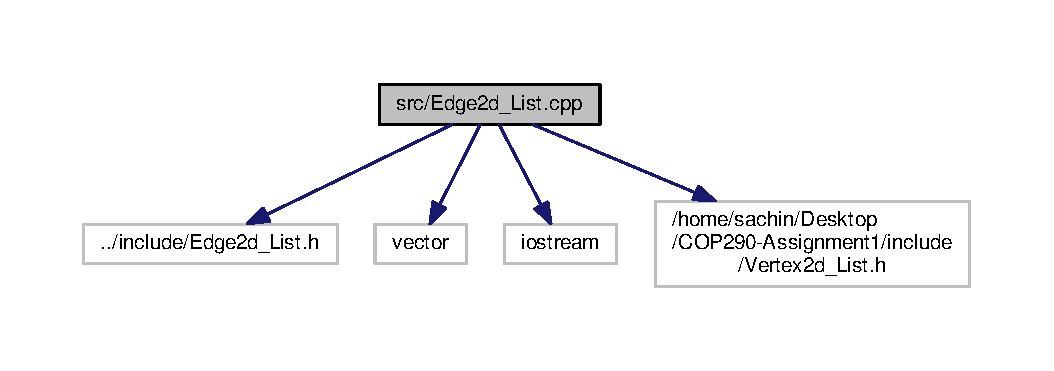
\includegraphics[width=350pt]{_edge2d___list_8cpp__incl}
\end{center}
\end{figure}
\subsection*{Functions}
\begin{DoxyCompactItemize}
\item 
bool \hyperlink{_edge2d___list_8cpp_adbe2c28fea9b36c2b6f4e2e88085511f}{equal\+\_\+2d\+Edge} (Edge2d e1, Edge2d e2)
\item 
bool \hyperlink{_edge2d___list_8cpp_aed13bf77691cc29b89b92f93239bba69}{parallel\+\_\+2d\+Edge} (Edge2d e1, Edge2d e2)
\item 
bool \hyperlink{_edge2d___list_8cpp_ade2cc17fcfffad19935d925902cf2d1f}{equal\+\_\+2dline} (Line2d line1, Line2d line2)
\item 
bool \hyperlink{_edge2d___list_8cpp_a61ab5cfb4252a679a6378dd492666fd5}{parallel\+\_\+2dline} (Line2d line1, Line2d line2)
\item 
bool \hyperlink{_edge2d___list_8cpp_ad85d2307300743c363e050904acbfbad}{equal\+\_\+direction} (Normal2d normal1, Normal2d normal2)
\item 
Vertex2d \hyperlink{_edge2d___list_8cpp_a73e1039d03e72e32386be4c1e0369578}{intersection\+\_\+of\+\_\+2dlines} (Line2d line1, Line2d line2)
\item 
Edge2d \hyperlink{_edge2d___list_8cpp_a12ae5fccb83db36e124e76387aa8cbd1}{union\+\_\+of\+\_\+two\+\_\+edges} (Edge2d edge2d1, Edge2d edge2d2)
\item 
int \hyperlink{_edge2d___list_8cpp_a3d765a5f17c461616342be113ce5a37a}{product\+\_\+of\+\_\+normal\+\_\+vertex\+\_\+in2d} (Normal2d normal, Vertex2d vertex)
\item 
float \hyperlink{_edge2d___list_8cpp_a8ee42a5dd83886e7ad61d451d5a32956}{min} (float a, float b)
\item 
float \hyperlink{_edge2d___list_8cpp_ac36750906e883bc6af51fbf3f251eb66}{max} (float a, float b)
\end{DoxyCompactItemize}


\subsection{Function Documentation}
\index{Edge2d\+\_\+\+List.\+cpp@{Edge2d\+\_\+\+List.\+cpp}!equal\+\_\+2d\+Edge@{equal\+\_\+2d\+Edge}}
\index{equal\+\_\+2d\+Edge@{equal\+\_\+2d\+Edge}!Edge2d\+\_\+\+List.\+cpp@{Edge2d\+\_\+\+List.\+cpp}}
\subsubsection[{\texorpdfstring{equal\+\_\+2d\+Edge(\+Edge2d e1, Edge2d e2)}{equal_2dEdge(Edge2d e1, Edge2d e2)}}]{\setlength{\rightskip}{0pt plus 5cm}bool equal\+\_\+2d\+Edge (
\begin{DoxyParamCaption}
\item[{Edge2d}]{e1, }
\item[{Edge2d}]{e2}
\end{DoxyParamCaption}
)}\hypertarget{_edge2d___list_8cpp_adbe2c28fea9b36c2b6f4e2e88085511f}{}\label{_edge2d___list_8cpp_adbe2c28fea9b36c2b6f4e2e88085511f}


Definition at line 153 of file Edge2d\+\_\+\+List.\+cpp.

\index{Edge2d\+\_\+\+List.\+cpp@{Edge2d\+\_\+\+List.\+cpp}!equal\+\_\+2dline@{equal\+\_\+2dline}}
\index{equal\+\_\+2dline@{equal\+\_\+2dline}!Edge2d\+\_\+\+List.\+cpp@{Edge2d\+\_\+\+List.\+cpp}}
\subsubsection[{\texorpdfstring{equal\+\_\+2dline(\+Line2d line1, Line2d line2)}{equal_2dline(Line2d line1, Line2d line2)}}]{\setlength{\rightskip}{0pt plus 5cm}bool equal\+\_\+2dline (
\begin{DoxyParamCaption}
\item[{Line2d}]{line1, }
\item[{Line2d}]{line2}
\end{DoxyParamCaption}
)}\hypertarget{_edge2d___list_8cpp_ade2cc17fcfffad19935d925902cf2d1f}{}\label{_edge2d___list_8cpp_ade2cc17fcfffad19935d925902cf2d1f}


Definition at line 163 of file Edge2d\+\_\+\+List.\+cpp.

\index{Edge2d\+\_\+\+List.\+cpp@{Edge2d\+\_\+\+List.\+cpp}!equal\+\_\+direction@{equal\+\_\+direction}}
\index{equal\+\_\+direction@{equal\+\_\+direction}!Edge2d\+\_\+\+List.\+cpp@{Edge2d\+\_\+\+List.\+cpp}}
\subsubsection[{\texorpdfstring{equal\+\_\+direction(\+Normal2d normal1, Normal2d normal2)}{equal_direction(Normal2d normal1, Normal2d normal2)}}]{\setlength{\rightskip}{0pt plus 5cm}bool equal\+\_\+direction (
\begin{DoxyParamCaption}
\item[{Normal2d}]{normal1, }
\item[{Normal2d}]{normal2}
\end{DoxyParamCaption}
)}\hypertarget{_edge2d___list_8cpp_ad85d2307300743c363e050904acbfbad}{}\label{_edge2d___list_8cpp_ad85d2307300743c363e050904acbfbad}


Definition at line 174 of file Edge2d\+\_\+\+List.\+cpp.

\index{Edge2d\+\_\+\+List.\+cpp@{Edge2d\+\_\+\+List.\+cpp}!intersection\+\_\+of\+\_\+2dlines@{intersection\+\_\+of\+\_\+2dlines}}
\index{intersection\+\_\+of\+\_\+2dlines@{intersection\+\_\+of\+\_\+2dlines}!Edge2d\+\_\+\+List.\+cpp@{Edge2d\+\_\+\+List.\+cpp}}
\subsubsection[{\texorpdfstring{intersection\+\_\+of\+\_\+2dlines(\+Line2d line1, Line2d line2)}{intersection_of_2dlines(Line2d line1, Line2d line2)}}]{\setlength{\rightskip}{0pt plus 5cm}Vertex2d intersection\+\_\+of\+\_\+2dlines (
\begin{DoxyParamCaption}
\item[{Line2d}]{line1, }
\item[{Line2d}]{line2}
\end{DoxyParamCaption}
)}\hypertarget{_edge2d___list_8cpp_a73e1039d03e72e32386be4c1e0369578}{}\label{_edge2d___list_8cpp_a73e1039d03e72e32386be4c1e0369578}


Definition at line 179 of file Edge2d\+\_\+\+List.\+cpp.

\index{Edge2d\+\_\+\+List.\+cpp@{Edge2d\+\_\+\+List.\+cpp}!max@{max}}
\index{max@{max}!Edge2d\+\_\+\+List.\+cpp@{Edge2d\+\_\+\+List.\+cpp}}
\subsubsection[{\texorpdfstring{max(float a, float b)}{max(float a, float b)}}]{\setlength{\rightskip}{0pt plus 5cm}float max (
\begin{DoxyParamCaption}
\item[{float}]{a, }
\item[{float}]{b}
\end{DoxyParamCaption}
)}\hypertarget{_edge2d___list_8cpp_ac36750906e883bc6af51fbf3f251eb66}{}\label{_edge2d___list_8cpp_ac36750906e883bc6af51fbf3f251eb66}


Definition at line 228 of file Edge2d\+\_\+\+List.\+cpp.

\index{Edge2d\+\_\+\+List.\+cpp@{Edge2d\+\_\+\+List.\+cpp}!min@{min}}
\index{min@{min}!Edge2d\+\_\+\+List.\+cpp@{Edge2d\+\_\+\+List.\+cpp}}
\subsubsection[{\texorpdfstring{min(float a, float b)}{min(float a, float b)}}]{\setlength{\rightskip}{0pt plus 5cm}float min (
\begin{DoxyParamCaption}
\item[{float}]{a, }
\item[{float}]{b}
\end{DoxyParamCaption}
)}\hypertarget{_edge2d___list_8cpp_a8ee42a5dd83886e7ad61d451d5a32956}{}\label{_edge2d___list_8cpp_a8ee42a5dd83886e7ad61d451d5a32956}


Definition at line 221 of file Edge2d\+\_\+\+List.\+cpp.

\index{Edge2d\+\_\+\+List.\+cpp@{Edge2d\+\_\+\+List.\+cpp}!parallel\+\_\+2d\+Edge@{parallel\+\_\+2d\+Edge}}
\index{parallel\+\_\+2d\+Edge@{parallel\+\_\+2d\+Edge}!Edge2d\+\_\+\+List.\+cpp@{Edge2d\+\_\+\+List.\+cpp}}
\subsubsection[{\texorpdfstring{parallel\+\_\+2d\+Edge(\+Edge2d e1, Edge2d e2)}{parallel_2dEdge(Edge2d e1, Edge2d e2)}}]{\setlength{\rightskip}{0pt plus 5cm}bool parallel\+\_\+2d\+Edge (
\begin{DoxyParamCaption}
\item[{Edge2d}]{e1, }
\item[{Edge2d}]{e2}
\end{DoxyParamCaption}
)}\hypertarget{_edge2d___list_8cpp_aed13bf77691cc29b89b92f93239bba69}{}\label{_edge2d___list_8cpp_aed13bf77691cc29b89b92f93239bba69}


Definition at line 158 of file Edge2d\+\_\+\+List.\+cpp.

\index{Edge2d\+\_\+\+List.\+cpp@{Edge2d\+\_\+\+List.\+cpp}!parallel\+\_\+2dline@{parallel\+\_\+2dline}}
\index{parallel\+\_\+2dline@{parallel\+\_\+2dline}!Edge2d\+\_\+\+List.\+cpp@{Edge2d\+\_\+\+List.\+cpp}}
\subsubsection[{\texorpdfstring{parallel\+\_\+2dline(\+Line2d line1, Line2d line2)}{parallel_2dline(Line2d line1, Line2d line2)}}]{\setlength{\rightskip}{0pt plus 5cm}bool parallel\+\_\+2dline (
\begin{DoxyParamCaption}
\item[{Line2d}]{line1, }
\item[{Line2d}]{line2}
\end{DoxyParamCaption}
)}\hypertarget{_edge2d___list_8cpp_a61ab5cfb4252a679a6378dd492666fd5}{}\label{_edge2d___list_8cpp_a61ab5cfb4252a679a6378dd492666fd5}


Definition at line 169 of file Edge2d\+\_\+\+List.\+cpp.

\index{Edge2d\+\_\+\+List.\+cpp@{Edge2d\+\_\+\+List.\+cpp}!product\+\_\+of\+\_\+normal\+\_\+vertex\+\_\+in2d@{product\+\_\+of\+\_\+normal\+\_\+vertex\+\_\+in2d}}
\index{product\+\_\+of\+\_\+normal\+\_\+vertex\+\_\+in2d@{product\+\_\+of\+\_\+normal\+\_\+vertex\+\_\+in2d}!Edge2d\+\_\+\+List.\+cpp@{Edge2d\+\_\+\+List.\+cpp}}
\subsubsection[{\texorpdfstring{product\+\_\+of\+\_\+normal\+\_\+vertex\+\_\+in2d(\+Normal2d normal, Vertex2d vertex)}{product_of_normal_vertex_in2d(Normal2d normal, Vertex2d vertex)}}]{\setlength{\rightskip}{0pt plus 5cm}int product\+\_\+of\+\_\+normal\+\_\+vertex\+\_\+in2d (
\begin{DoxyParamCaption}
\item[{Normal2d}]{normal, }
\item[{Vertex2d}]{vertex}
\end{DoxyParamCaption}
)}\hypertarget{_edge2d___list_8cpp_a3d765a5f17c461616342be113ce5a37a}{}\label{_edge2d___list_8cpp_a3d765a5f17c461616342be113ce5a37a}


Definition at line 217 of file Edge2d\+\_\+\+List.\+cpp.

\index{Edge2d\+\_\+\+List.\+cpp@{Edge2d\+\_\+\+List.\+cpp}!union\+\_\+of\+\_\+two\+\_\+edges@{union\+\_\+of\+\_\+two\+\_\+edges}}
\index{union\+\_\+of\+\_\+two\+\_\+edges@{union\+\_\+of\+\_\+two\+\_\+edges}!Edge2d\+\_\+\+List.\+cpp@{Edge2d\+\_\+\+List.\+cpp}}
\subsubsection[{\texorpdfstring{union\+\_\+of\+\_\+two\+\_\+edges(\+Edge2d edge2d1, Edge2d edge2d2)}{union_of_two_edges(Edge2d edge2d1, Edge2d edge2d2)}}]{\setlength{\rightskip}{0pt plus 5cm}Edge2d union\+\_\+of\+\_\+two\+\_\+edges (
\begin{DoxyParamCaption}
\item[{Edge2d}]{edge2d1, }
\item[{Edge2d}]{edge2d2}
\end{DoxyParamCaption}
)}\hypertarget{_edge2d___list_8cpp_a12ae5fccb83db36e124e76387aa8cbd1}{}\label{_edge2d___list_8cpp_a12ae5fccb83db36e124e76387aa8cbd1}


Definition at line 192 of file Edge2d\+\_\+\+List.\+cpp.


\hypertarget{_edge3d___list_8cpp}{}\section{src/\+Edge3d\+\_\+\+List.cpp File Reference}
\label{_edge3d___list_8cpp}\index{src/\+Edge3d\+\_\+\+List.\+cpp@{src/\+Edge3d\+\_\+\+List.\+cpp}}
{\ttfamily \#include \char`\"{}../include/\+Edge3d\+\_\+\+List.\+h\char`\"{}}\\*
Include dependency graph for Edge3d\+\_\+\+List.\+cpp\+:\nopagebreak
\begin{figure}[H]
\begin{center}
\leavevmode
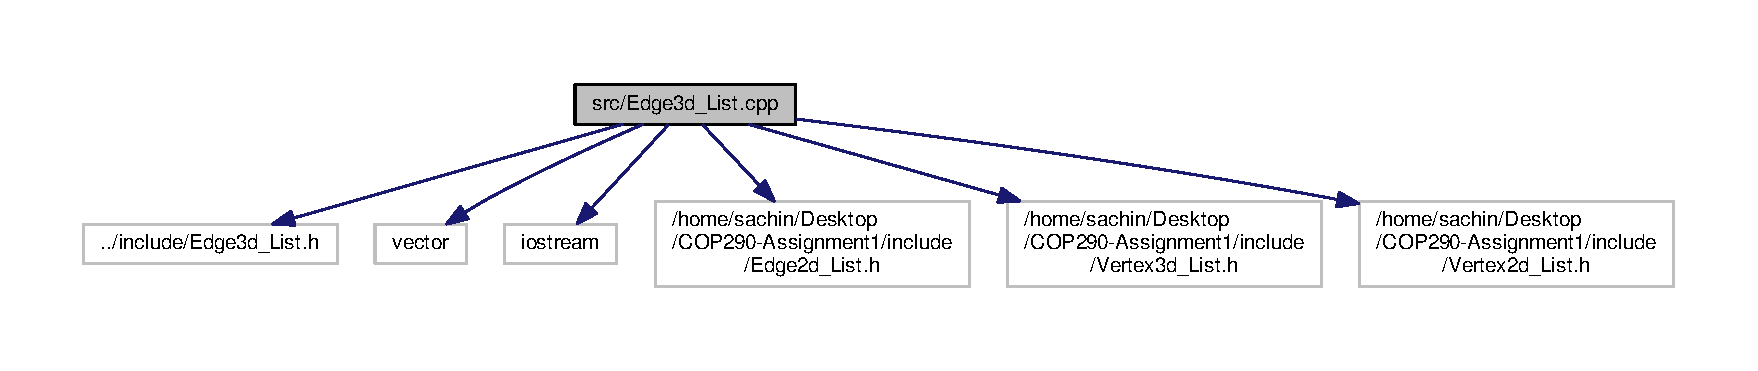
\includegraphics[width=350pt]{_edge3d___list_8cpp__incl}
\end{center}
\end{figure}
\subsection*{Namespaces}
\begin{DoxyCompactItemize}
\item 
 \hyperlink{namespaceextra__functions__3dedge}{extra\+\_\+functions\+\_\+3dedge}
\end{DoxyCompactItemize}
\subsection*{Functions}
\begin{DoxyCompactItemize}
\item 
bool \hyperlink{namespaceextra__functions__3dedge_ae7c8fa0d6b3476fe882e957553ccdd86}{extra\+\_\+functions\+\_\+3dedge\+::equal\+\_\+3dedge} (Edge3d e1, Edge3d e2)
\item 
int \hyperlink{namespaceextra__functions__3dedge_a5ad68cbd008f410b737b334315042d56}{extra\+\_\+functions\+\_\+3dedge\+::edge\+\_\+index} (vector$<$ Edge3d $>$ elist, Edge3d e)
\end{DoxyCompactItemize}

\hypertarget{_face3d___list_8cpp}{}\section{src/\+Face3d\+\_\+\+List.cpp File Reference}
\label{_face3d___list_8cpp}\index{src/\+Face3d\+\_\+\+List.\+cpp@{src/\+Face3d\+\_\+\+List.\+cpp}}
{\ttfamily \#include \char`\"{}../include/\+Face3d\+\_\+\+List.\+h\char`\"{}}\\*
Include dependency graph for Face3d\+\_\+\+List.\+cpp\+:\nopagebreak
\begin{figure}[H]
\begin{center}
\leavevmode
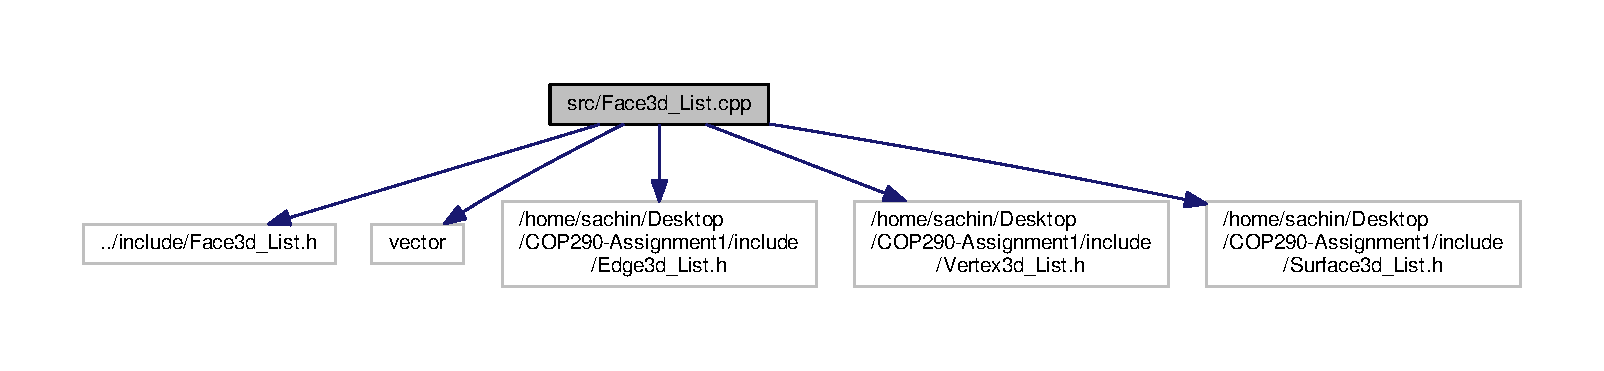
\includegraphics[width=350pt]{_face3d___list_8cpp__incl}
\end{center}
\end{figure}

\hypertarget{_hidden_lines_8cpp}{}\section{src/\+Hidden\+Lines.cpp File Reference}
\label{_hidden_lines_8cpp}\index{src/\+Hidden\+Lines.\+cpp@{src/\+Hidden\+Lines.\+cpp}}
{\ttfamily \#include \char`\"{}../include/\+Hidden\+Lines.\+h\char`\"{}}\\*
Include dependency graph for Hidden\+Lines.\+cpp\+:\nopagebreak
\begin{figure}[H]
\begin{center}
\leavevmode
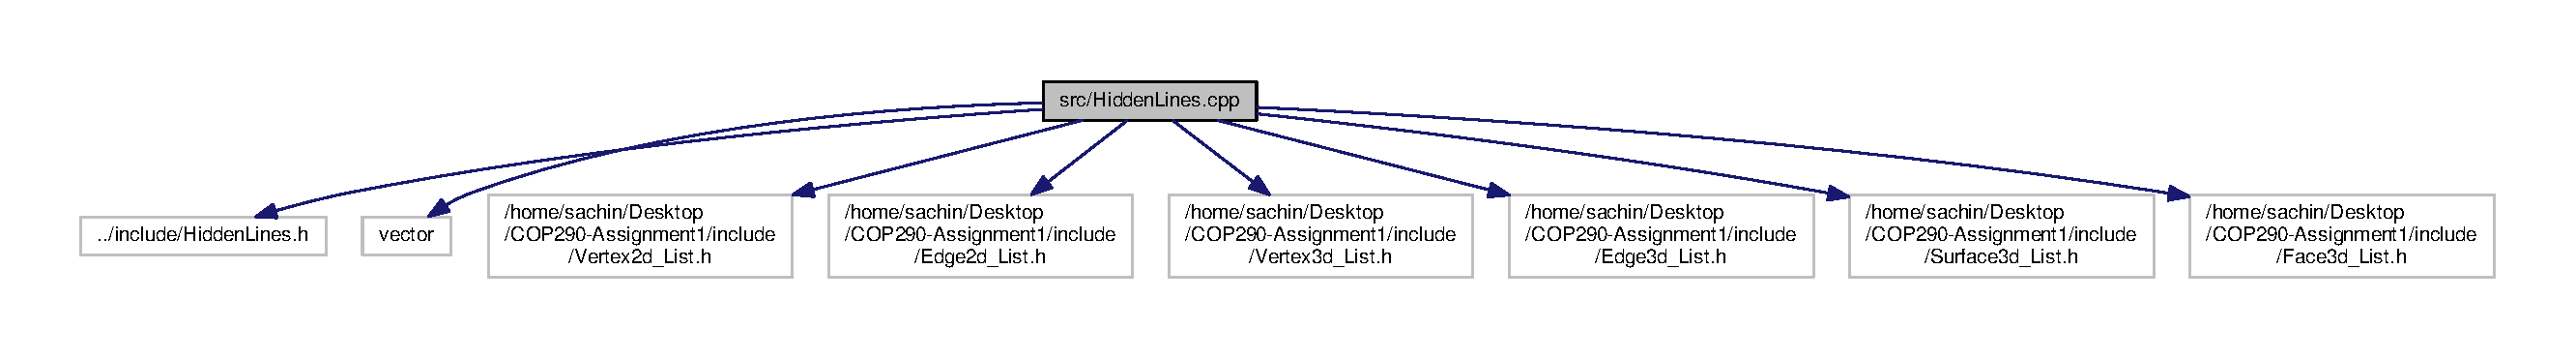
\includegraphics[width=350pt]{_hidden_lines_8cpp__incl}
\end{center}
\end{figure}

\hypertarget{main_8cpp}{}\section{src/main.cpp File Reference}
\label{main_8cpp}\index{src/main.\+cpp@{src/main.\+cpp}}
{\ttfamily \#include $<$iostream$>$}\\*
{\ttfamily \#include \char`\"{}../include/\+Edge3d\+\_\+\+List.\+h\char`\"{}}\\*
{\ttfamily \#include \char`\"{}../include/\+Edge2d\+\_\+\+List.\+h\char`\"{}}\\*
{\ttfamily \#include \char`\"{}../include/\+Hidden\+Lines.\+h\char`\"{}}\\*
{\ttfamily \#include \char`\"{}../include/\+Projection2d.\+h\char`\"{}}\\*
{\ttfamily \#include \char`\"{}../include/\+Solid3d.\+h\char`\"{}}\\*
{\ttfamily \#include \char`\"{}../include/\+Surface3d\+\_\+\+List.\+h\char`\"{}}\\*
{\ttfamily \#include \char`\"{}../include/\+Vertex2d\+\_\+\+List.\+h\char`\"{}}\\*
{\ttfamily \#include \char`\"{}../include/\+Vertex3d\+\_\+\+List.\+h\char`\"{}}\\*
{\ttfamily \#include $<$math.\+h$>$}\\*
{\ttfamily \#include $<$Qt\+Core$>$}\\*
{\ttfamily \#include $<$Qt\+Gui$>$}\\*
{\ttfamily \#include $<$stdlib.\+h$>$}\\*
Include dependency graph for main.\+cpp\+:\nopagebreak
\begin{figure}[H]
\begin{center}
\leavevmode
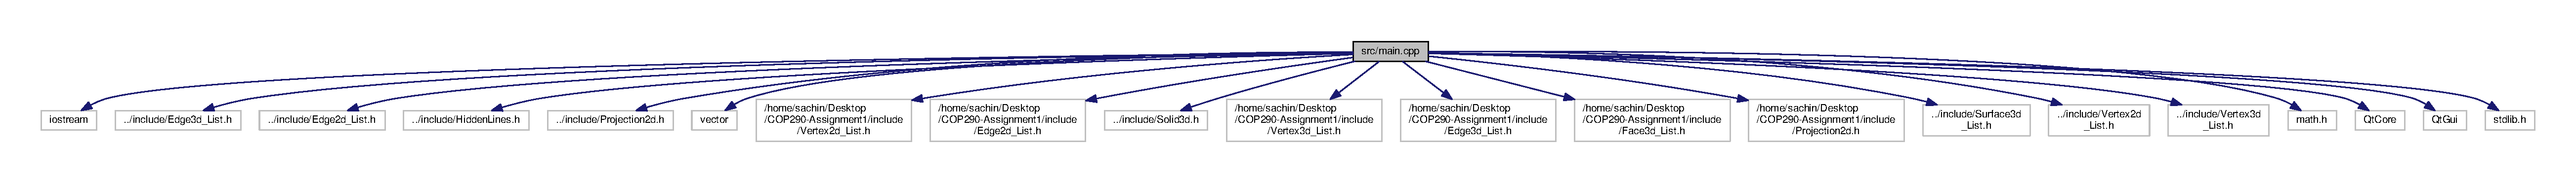
\includegraphics[width=350pt]{main_8cpp__incl}
\end{center}
\end{figure}
\subsection*{Macros}
\begin{DoxyCompactItemize}
\item 
\#define \hyperlink{main_8cpp_a598a3330b3c21701223ee0ca14316eca}{PI}~3.\+1415926536
\item 
\#define \hyperlink{main_8cpp_a70ed59adcb4159ac551058053e649640}{S\+I\+ZE}~200
\item 
\#define \hyperlink{main_8cpp_a63c7acef5369ac4e5fd5f852ee1720e0}{F\+A\+C\+T\+OR}~100
\end{DoxyCompactItemize}
\subsection*{Functions}
\begin{DoxyCompactItemize}
\item 
void \hyperlink{main_8cpp_a2858154e2009b0e6e616f313177762bc}{init} (void)
\item 
void \hyperlink{main_8cpp_a4ea013001a5fb47853d0fab8f8de35cd}{display} (void)
\item 
int \hyperlink{main_8cpp_a0ddf1224851353fc92bfbff6f499fa97}{main} (int argc, char $\ast$argv\mbox{[}$\,$\mbox{]})
\end{DoxyCompactItemize}
\subsection*{Variables}
\begin{DoxyCompactItemize}
\item 
const float \hyperlink{main_8cpp_a22a8bcfa9f0309676ac74f599b2bbd39}{S\+T\+EP} = 2$\ast$\hyperlink{main_8cpp_a598a3330b3c21701223ee0ca14316eca}{PI}/\hyperlink{main_8cpp_a70ed59adcb4159ac551058053e649640}{S\+I\+ZE}
\item 
Edge2d\+\_\+\+List \hyperlink{main_8cpp_a2d213a7b47b460d6939b6dd4510a905b}{ex}
\end{DoxyCompactItemize}


\subsection{Macro Definition Documentation}
\index{main.\+cpp@{main.\+cpp}!F\+A\+C\+T\+OR@{F\+A\+C\+T\+OR}}
\index{F\+A\+C\+T\+OR@{F\+A\+C\+T\+OR}!main.\+cpp@{main.\+cpp}}
\subsubsection[{\texorpdfstring{F\+A\+C\+T\+OR}{FACTOR}}]{\setlength{\rightskip}{0pt plus 5cm}\#define F\+A\+C\+T\+OR~100}\hypertarget{main_8cpp_a63c7acef5369ac4e5fd5f852ee1720e0}{}\label{main_8cpp_a63c7acef5369ac4e5fd5f852ee1720e0}


Definition at line 19 of file main.\+cpp.

\index{main.\+cpp@{main.\+cpp}!PI@{PI}}
\index{PI@{PI}!main.\+cpp@{main.\+cpp}}
\subsubsection[{\texorpdfstring{PI}{PI}}]{\setlength{\rightskip}{0pt plus 5cm}\#define PI~3.\+1415926536}\hypertarget{main_8cpp_a598a3330b3c21701223ee0ca14316eca}{}\label{main_8cpp_a598a3330b3c21701223ee0ca14316eca}


Definition at line 17 of file main.\+cpp.

\index{main.\+cpp@{main.\+cpp}!S\+I\+ZE@{S\+I\+ZE}}
\index{S\+I\+ZE@{S\+I\+ZE}!main.\+cpp@{main.\+cpp}}
\subsubsection[{\texorpdfstring{S\+I\+ZE}{SIZE}}]{\setlength{\rightskip}{0pt plus 5cm}\#define S\+I\+ZE~200}\hypertarget{main_8cpp_a70ed59adcb4159ac551058053e649640}{}\label{main_8cpp_a70ed59adcb4159ac551058053e649640}


Definition at line 18 of file main.\+cpp.



\subsection{Function Documentation}
\index{main.\+cpp@{main.\+cpp}!display@{display}}
\index{display@{display}!main.\+cpp@{main.\+cpp}}
\subsubsection[{\texorpdfstring{display(void)}{display(void)}}]{\setlength{\rightskip}{0pt plus 5cm}void display (
\begin{DoxyParamCaption}
\item[{void}]{}
\end{DoxyParamCaption}
)}\hypertarget{main_8cpp_a4ea013001a5fb47853d0fab8f8de35cd}{}\label{main_8cpp_a4ea013001a5fb47853d0fab8f8de35cd}
\index{main.\+cpp@{main.\+cpp}!init@{init}}
\index{init@{init}!main.\+cpp@{main.\+cpp}}
\subsubsection[{\texorpdfstring{init(void)}{init(void)}}]{\setlength{\rightskip}{0pt plus 5cm}void init (
\begin{DoxyParamCaption}
\item[{void}]{}
\end{DoxyParamCaption}
)}\hypertarget{main_8cpp_a2858154e2009b0e6e616f313177762bc}{}\label{main_8cpp_a2858154e2009b0e6e616f313177762bc}
\index{main.\+cpp@{main.\+cpp}!main@{main}}
\index{main@{main}!main.\+cpp@{main.\+cpp}}
\subsubsection[{\texorpdfstring{main(int argc, char $\ast$argv[])}{main(int argc, char *argv[])}}]{\setlength{\rightskip}{0pt plus 5cm}int main (
\begin{DoxyParamCaption}
\item[{int}]{argc, }
\item[{char $\ast$}]{argv\mbox{[}$\,$\mbox{]}}
\end{DoxyParamCaption}
)}\hypertarget{main_8cpp_a0ddf1224851353fc92bfbff6f499fa97}{}\label{main_8cpp_a0ddf1224851353fc92bfbff6f499fa97}


Definition at line 29 of file main.\+cpp.



\subsection{Variable Documentation}
\index{main.\+cpp@{main.\+cpp}!ex@{ex}}
\index{ex@{ex}!main.\+cpp@{main.\+cpp}}
\subsubsection[{\texorpdfstring{ex}{ex}}]{\setlength{\rightskip}{0pt plus 5cm}Edge2d\+\_\+\+List ex}\hypertarget{main_8cpp_a2d213a7b47b460d6939b6dd4510a905b}{}\label{main_8cpp_a2d213a7b47b460d6939b6dd4510a905b}


Definition at line 27 of file main.\+cpp.

\index{main.\+cpp@{main.\+cpp}!S\+T\+EP@{S\+T\+EP}}
\index{S\+T\+EP@{S\+T\+EP}!main.\+cpp@{main.\+cpp}}
\subsubsection[{\texorpdfstring{S\+T\+EP}{STEP}}]{\setlength{\rightskip}{0pt plus 5cm}const float S\+T\+EP = 2$\ast${\bf PI}/{\bf S\+I\+ZE}}\hypertarget{main_8cpp_a22a8bcfa9f0309676ac74f599b2bbd39}{}\label{main_8cpp_a22a8bcfa9f0309676ac74f599b2bbd39}


Definition at line 21 of file main.\+cpp.


\hypertarget{_projection2d_8cpp}{}\section{src/\+Projection2d.cpp File Reference}
\label{_projection2d_8cpp}\index{src/\+Projection2d.\+cpp@{src/\+Projection2d.\+cpp}}
{\ttfamily \#include \char`\"{}../include/\+Projection2d.\+h\char`\"{}}\\*
Include dependency graph for Projection2d.\+cpp\+:\nopagebreak
\begin{figure}[H]
\begin{center}
\leavevmode
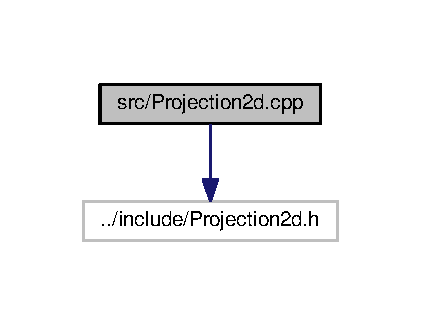
\includegraphics[width=202pt]{_projection2d_8cpp__incl}
\end{center}
\end{figure}

\hypertarget{_solid3d_8cpp}{}\section{src/\+Solid3d.cpp File Reference}
\label{_solid3d_8cpp}\index{src/\+Solid3d.\+cpp@{src/\+Solid3d.\+cpp}}
{\ttfamily \#include \char`\"{}../include/\+Solid3d.\+h\char`\"{}}\\*
Include dependency graph for Solid3d.\+cpp\+:\nopagebreak
\begin{figure}[H]
\begin{center}
\leavevmode
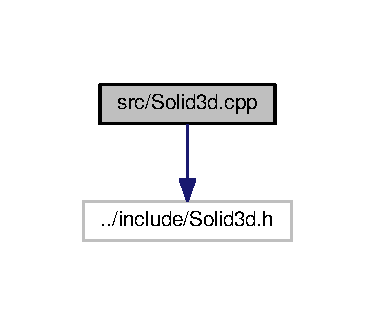
\includegraphics[width=180pt]{_solid3d_8cpp__incl}
\end{center}
\end{figure}

\hypertarget{_surface3d___list_8cpp}{}\section{src/\+Surface3d\+\_\+\+List.cpp File Reference}
\label{_surface3d___list_8cpp}\index{src/\+Surface3d\+\_\+\+List.\+cpp@{src/\+Surface3d\+\_\+\+List.\+cpp}}
{\ttfamily \#include \char`\"{}../include/\+Surface3d\+\_\+\+List.\+h\char`\"{}}\\*
Include dependency graph for Surface3d\+\_\+\+List.\+cpp\+:\nopagebreak
\begin{figure}[H]
\begin{center}
\leavevmode
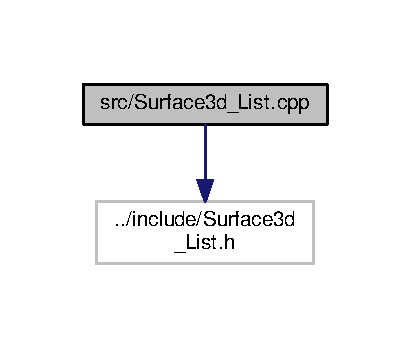
\includegraphics[width=197pt]{_surface3d___list_8cpp__incl}
\end{center}
\end{figure}
\subsection*{Functions}
\begin{DoxyCompactItemize}
\item 
bool \hyperlink{_surface3d___list_8cpp_a114c9d2d3c26cd8a9a9366fbae8ef7a7}{equal\+\_\+normals} (Normal3d normal1, Normal3d normal2)
\item 
bool \hyperlink{_surface3d___list_8cpp_a18677c7673880cd0130b98c624e7c41e}{equal\+\_\+3dsurface} (Surface3d surface1, Surface3d surface2)
\item 
int \hyperlink{_surface3d___list_8cpp_a8deee00992489ff360c3407ed2fa2bee}{dot\+\_\+product\+\_\+of\+\_\+normals} (Normal3d normal1, Normal3d normal2)
\item 
int \hyperlink{_surface3d___list_8cpp_a8e2efd5488b1f0a20a81248b6773a8ac}{product\+\_\+of\+\_\+normal\+\_\+vertex\+\_\+in3d} (Normal3d normal, Vertex3d vertex)
\end{DoxyCompactItemize}


\subsection{Function Documentation}
\index{Surface3d\+\_\+\+List.\+cpp@{Surface3d\+\_\+\+List.\+cpp}!dot\+\_\+product\+\_\+of\+\_\+normals@{dot\+\_\+product\+\_\+of\+\_\+normals}}
\index{dot\+\_\+product\+\_\+of\+\_\+normals@{dot\+\_\+product\+\_\+of\+\_\+normals}!Surface3d\+\_\+\+List.\+cpp@{Surface3d\+\_\+\+List.\+cpp}}
\subsubsection[{\texorpdfstring{dot\+\_\+product\+\_\+of\+\_\+normals(\+Normal3d normal1, Normal3d normal2)}{dot_product_of_normals(Normal3d normal1, Normal3d normal2)}}]{\setlength{\rightskip}{0pt plus 5cm}int dot\+\_\+product\+\_\+of\+\_\+normals (
\begin{DoxyParamCaption}
\item[{Normal3d}]{normal1, }
\item[{Normal3d}]{normal2}
\end{DoxyParamCaption}
)}\hypertarget{_surface3d___list_8cpp_a8deee00992489ff360c3407ed2fa2bee}{}\label{_surface3d___list_8cpp_a8deee00992489ff360c3407ed2fa2bee}


Definition at line 114 of file Surface3d\+\_\+\+List.\+cpp.

\index{Surface3d\+\_\+\+List.\+cpp@{Surface3d\+\_\+\+List.\+cpp}!equal\+\_\+3dsurface@{equal\+\_\+3dsurface}}
\index{equal\+\_\+3dsurface@{equal\+\_\+3dsurface}!Surface3d\+\_\+\+List.\+cpp@{Surface3d\+\_\+\+List.\+cpp}}
\subsubsection[{\texorpdfstring{equal\+\_\+3dsurface(\+Surface3d surface1, Surface3d surface2)}{equal_3dsurface(Surface3d surface1, Surface3d surface2)}}]{\setlength{\rightskip}{0pt plus 5cm}bool equal\+\_\+3dsurface (
\begin{DoxyParamCaption}
\item[{Surface3d}]{surface1, }
\item[{Surface3d}]{surface2}
\end{DoxyParamCaption}
)}\hypertarget{_surface3d___list_8cpp_a18677c7673880cd0130b98c624e7c41e}{}\label{_surface3d___list_8cpp_a18677c7673880cd0130b98c624e7c41e}


Definition at line 103 of file Surface3d\+\_\+\+List.\+cpp.

\index{Surface3d\+\_\+\+List.\+cpp@{Surface3d\+\_\+\+List.\+cpp}!equal\+\_\+normals@{equal\+\_\+normals}}
\index{equal\+\_\+normals@{equal\+\_\+normals}!Surface3d\+\_\+\+List.\+cpp@{Surface3d\+\_\+\+List.\+cpp}}
\subsubsection[{\texorpdfstring{equal\+\_\+normals(\+Normal3d normal1, Normal3d normal2)}{equal_normals(Normal3d normal1, Normal3d normal2)}}]{\setlength{\rightskip}{0pt plus 5cm}bool equal\+\_\+normals (
\begin{DoxyParamCaption}
\item[{Normal3d}]{normal1, }
\item[{Normal3d}]{normal2}
\end{DoxyParamCaption}
)}\hypertarget{_surface3d___list_8cpp_a114c9d2d3c26cd8a9a9366fbae8ef7a7}{}\label{_surface3d___list_8cpp_a114c9d2d3c26cd8a9a9366fbae8ef7a7}


Definition at line 97 of file Surface3d\+\_\+\+List.\+cpp.

\index{Surface3d\+\_\+\+List.\+cpp@{Surface3d\+\_\+\+List.\+cpp}!product\+\_\+of\+\_\+normal\+\_\+vertex\+\_\+in3d@{product\+\_\+of\+\_\+normal\+\_\+vertex\+\_\+in3d}}
\index{product\+\_\+of\+\_\+normal\+\_\+vertex\+\_\+in3d@{product\+\_\+of\+\_\+normal\+\_\+vertex\+\_\+in3d}!Surface3d\+\_\+\+List.\+cpp@{Surface3d\+\_\+\+List.\+cpp}}
\subsubsection[{\texorpdfstring{product\+\_\+of\+\_\+normal\+\_\+vertex\+\_\+in3d(\+Normal3d normal, Vertex3d vertex)}{product_of_normal_vertex_in3d(Normal3d normal, Vertex3d vertex)}}]{\setlength{\rightskip}{0pt plus 5cm}int product\+\_\+of\+\_\+normal\+\_\+vertex\+\_\+in3d (
\begin{DoxyParamCaption}
\item[{Normal3d}]{normal, }
\item[{Vertex3d}]{vertex}
\end{DoxyParamCaption}
)}\hypertarget{_surface3d___list_8cpp_a8e2efd5488b1f0a20a81248b6773a8ac}{}\label{_surface3d___list_8cpp_a8e2efd5488b1f0a20a81248b6773a8ac}


Definition at line 119 of file Surface3d\+\_\+\+List.\+cpp.


\hypertarget{_vertex2d___list_8cpp}{}\section{src/\+Vertex2d\+\_\+\+List.cpp File Reference}
\label{_vertex2d___list_8cpp}\index{src/\+Vertex2d\+\_\+\+List.\+cpp@{src/\+Vertex2d\+\_\+\+List.\+cpp}}
{\ttfamily \#include \char`\"{}../include/\+Vertex2d\+\_\+\+List.\+h\char`\"{}}\\*
Include dependency graph for Vertex2d\+\_\+\+List.\+cpp\+:\nopagebreak
\begin{figure}[H]
\begin{center}
\leavevmode
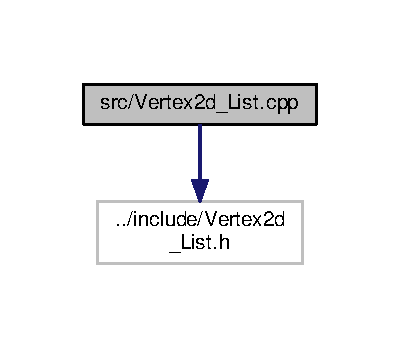
\includegraphics[width=192pt]{_vertex2d___list_8cpp__incl}
\end{center}
\end{figure}
\subsection*{Functions}
\begin{DoxyCompactItemize}
\item 
bool \hyperlink{_vertex2d___list_8cpp_a53328f6247e2c83ed5bdac22d2d511ab}{equal\+\_\+2d\+Vertex} (Vertex2d v1, Vertex2d v2)
\item 
int \hyperlink{_vertex2d___list_8cpp_a567eeaf8de62b3db14c480e49841455d}{vertex\+\_\+indexin2d} (vector$<$ Vertex2d $>$ vlist, Vertex2d v)
\end{DoxyCompactItemize}
\subsection*{Variables}
\begin{DoxyCompactItemize}
\item 
int \hyperlink{_vertex2d___list_8cpp_a4dc1dc65750ded2342bb4aef5a4b9326}{D\+E\+L\+TA} = 0
\end{DoxyCompactItemize}


\subsection{Function Documentation}
\index{Vertex2d\+\_\+\+List.\+cpp@{Vertex2d\+\_\+\+List.\+cpp}!equal\+\_\+2d\+Vertex@{equal\+\_\+2d\+Vertex}}
\index{equal\+\_\+2d\+Vertex@{equal\+\_\+2d\+Vertex}!Vertex2d\+\_\+\+List.\+cpp@{Vertex2d\+\_\+\+List.\+cpp}}
\subsubsection[{\texorpdfstring{equal\+\_\+2d\+Vertex(\+Vertex2d v1, Vertex2d v2)}{equal_2dVertex(Vertex2d v1, Vertex2d v2)}}]{\setlength{\rightskip}{0pt plus 5cm}bool equal\+\_\+2d\+Vertex (
\begin{DoxyParamCaption}
\item[{Vertex2d}]{v1, }
\item[{Vertex2d}]{v2}
\end{DoxyParamCaption}
)}\hypertarget{_vertex2d___list_8cpp_a53328f6247e2c83ed5bdac22d2d511ab}{}\label{_vertex2d___list_8cpp_a53328f6247e2c83ed5bdac22d2d511ab}


Definition at line 69 of file Vertex2d\+\_\+\+List.\+cpp.

\index{Vertex2d\+\_\+\+List.\+cpp@{Vertex2d\+\_\+\+List.\+cpp}!vertex\+\_\+indexin2d@{vertex\+\_\+indexin2d}}
\index{vertex\+\_\+indexin2d@{vertex\+\_\+indexin2d}!Vertex2d\+\_\+\+List.\+cpp@{Vertex2d\+\_\+\+List.\+cpp}}
\subsubsection[{\texorpdfstring{vertex\+\_\+indexin2d(vector$<$ Vertex2d $>$ vlist, Vertex2d v)}{vertex_indexin2d(vector< Vertex2d > vlist, Vertex2d v)}}]{\setlength{\rightskip}{0pt plus 5cm}int vertex\+\_\+indexin2d (
\begin{DoxyParamCaption}
\item[{vector$<$ Vertex2d $>$}]{vlist, }
\item[{Vertex2d}]{v}
\end{DoxyParamCaption}
)}\hypertarget{_vertex2d___list_8cpp_a567eeaf8de62b3db14c480e49841455d}{}\label{_vertex2d___list_8cpp_a567eeaf8de62b3db14c480e49841455d}


Definition at line 73 of file Vertex2d\+\_\+\+List.\+cpp.



\subsection{Variable Documentation}
\index{Vertex2d\+\_\+\+List.\+cpp@{Vertex2d\+\_\+\+List.\+cpp}!D\+E\+L\+TA@{D\+E\+L\+TA}}
\index{D\+E\+L\+TA@{D\+E\+L\+TA}!Vertex2d\+\_\+\+List.\+cpp@{Vertex2d\+\_\+\+List.\+cpp}}
\subsubsection[{\texorpdfstring{D\+E\+L\+TA}{DELTA}}]{\setlength{\rightskip}{0pt plus 5cm}int D\+E\+L\+TA = 0}\hypertarget{_vertex2d___list_8cpp_a4dc1dc65750ded2342bb4aef5a4b9326}{}\label{_vertex2d___list_8cpp_a4dc1dc65750ded2342bb4aef5a4b9326}


Definition at line 5 of file Vertex2d\+\_\+\+List.\+cpp.


\hypertarget{_vertex3d___list_8cpp}{}\section{src/\+Vertex3d\+\_\+\+List.cpp File Reference}
\label{_vertex3d___list_8cpp}\index{src/\+Vertex3d\+\_\+\+List.\+cpp@{src/\+Vertex3d\+\_\+\+List.\+cpp}}
{\ttfamily \#include \char`\"{}../include/\+Vertex3d\+\_\+\+List.\+h\char`\"{}}\\*
Include dependency graph for Vertex3d\+\_\+\+List.\+cpp\+:\nopagebreak
\begin{figure}[H]
\begin{center}
\leavevmode
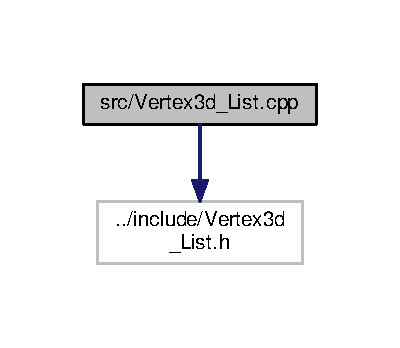
\includegraphics[width=192pt]{_vertex3d___list_8cpp__incl}
\end{center}
\end{figure}
\subsection*{Namespaces}
\begin{DoxyCompactItemize}
\item 
 \hyperlink{namespaceextra__functions__3dvertex}{extra\+\_\+functions\+\_\+3dvertex}
\end{DoxyCompactItemize}
\subsection*{Functions}
\begin{DoxyCompactItemize}
\item 
bool \hyperlink{namespaceextra__functions__3dvertex_a0da949fe0a7c4031ef70dc6f95145845}{extra\+\_\+functions\+\_\+3dvertex\+::vertex3d\+\_\+possible} (Vertex2d front, Vertex2d top, Vertex2d side)
\item 
bool \hyperlink{namespaceextra__functions__3dvertex_a9428b2b2156e274aff497ebd80f5e3a1}{extra\+\_\+functions\+\_\+3dvertex\+::equal\+\_\+3dvertex} (Vertex3d v1, Vertex3d v2)
\item 
Vertex3d \hyperlink{namespaceextra__functions__3dvertex_a8016663b5ddeb59267c20901a5e26946}{extra\+\_\+functions\+\_\+3dvertex\+::vertex3d\+\_\+generate} (Vertex2d front, Vertex2d top, Vertex2d side)
\item 
vector$<$ Vertex3d $>$ \hyperlink{namespaceextra__functions__3dvertex_a63195c28bf72d9d5b22965c492c58f16}{extra\+\_\+functions\+\_\+3dvertex\+::vertex3dlist\+\_\+generate} (Vertex2d\+\_\+\+List front\+\_\+list, Vertex2d\+\_\+\+List top\+\_\+list, Vertex2d\+\_\+\+List side\+\_\+list)
\item 
int \hyperlink{namespaceextra__functions__3dvertex_a90d4205a4176bda11a8c2212d70268fc}{extra\+\_\+functions\+\_\+3dvertex\+::vertex\+\_\+index} (vector$<$ Vertex3d $>$ vlist, Vertex3d v)
\end{DoxyCompactItemize}

%--- End generated contents ---

% Index
\backmatter
\newpage
\phantomsection
\clearemptydoublepage
\addcontentsline{toc}{chapter}{Index}
\printindex

\end{document}
